
\setcounter{chapter}{3}
\chapter{Library Applications and Evaluation}
\minitoc %insert la minitoc
\graphicspath{{Chapitre4/figures/}}

%\DoPToC
%==============================================================================
\pagestyle{fancy}
\fancyhf{}
\fancyhead[R]{\bfseries\rightmark}
\fancyfoot[R]{\thepage}
\renewcommand{\headrulewidth}{0.5pt}
\renewcommand{\footrulewidth}{0pt}
\renewcommand{\chaptermark}[1]{\markboth{{\chaptername~\thechapter. #1 }}{}}
\renewcommand{\sectionmark}[1]{\markright{\thechapter.\thesection~ #1}}

\begin{spacing}{1.2}

    %==============================================================================
    \section*{Introduction}
    In previous chapters, we went through the high level architecture and the implementation of the library. In this chapter,
    we will explore how the components of the library can be combined to realize different use cases. We will also discuss
    the parallelization features of the library and how it can be used to improve the performance of the applications.
    Finally, we will present the results of the performance evaluation of the library.

    \section{Examples of Library Applications}
    \subsection{Receive frames, Analyze data, Save results}
    First, we will go through a basic but very common example of using the library. A typical use case
    of the library is to listen to the slsReceiver for frames, run the cluster finder on the frames as they come in,
    and store the results in a local file.
    This example combines the four modules of the library: core, file\_io, network\_io and processing.
    The code snippet below \ref{lst:listen_analyze_store} shows how this can be done in a few lines of code.

    \begin{lstlisting}[language=C++, caption=Example of a common use case ,label=lst:listen_analyze_store]
ZmqSocketReceiver receiver("tcp://localhost:5555");
receiver.connect(); // connect to slsReceiver
ClusterFinder clusterFinder(3,3); // 3x3 cluster
ClusterFile clusterFile("clusters.txt","w"); // write to cluster file
Pedestal pedestal(512,512,1000); // pedestal with size 512x512 and averages over last 1000 frames

while(true){
    // receive a frame
    ZmqFrame zmq_frame = receiver.receive_zmqframe();
    Frame frame = zmq_frame.frame;
    // find clusters in the frame
    std::vector<DynamicCluster> clusters = clusterFinder.find_clusters_without_threshold(frame,pedestal);
    // write clusters to file
    ClusterHeader header = {frame.header, clusters.size()};
    clusterFile.write(header, clusters);
}    
\end{lstlisting}

    The library provides a high level interface to the user, abstracting a lot of the implementation
    details. The scientist can focus on the data analysis part of the code while the library
    provides reliable, efficient and potent tools to handle the rest.
    \subsection{File Streaming}
    Another common use case is to read frames from a file and stream them to one or multiple
    receivers. This can be useful for testing the performance of the library or for debugging.
    The file streamer can integrate with other existing systems such as GUI applications or
    data processing pipelines.
    \begin{lstlisting}[language=C++, caption=Example of file streaming ,label=lst:file_streaming]
File file("data_master.json"); // open file for reading
ZmqSocketSender sender("tcp://*:5555"); // create a socket to send frames
sender.bind(); // bind to port 5555
// iterate over all frames in the file
for(int i=0; i<file.total_frames(); i++){
    Frame frame = file.read_frame(); // get frame
    // create a header and fill its metadata
    ZmqHeader header;
    header.frame_number = i;
    // create a zmq frame and send it
    ZmqFrame zmq_frame = {header, frame};
    sender.send_zmqframe(zmq_frame);
}
        
    \end{lstlisting}

    \subsection{Load Balancer}
    As the detector technology evolves, the data rates are increasing. Scaling vertically
    by increasing the processing power of a single machine is a good solution but it can
    only go so far. Scaling horizontally by adding more machines to the processing pipeline
    is a more sustainable solution. As explained in the previous chapter
    \ref{fig:task_distribution} \ref{lst:task_ventilator} \ref{lst:task_worker} \ref{lst:task_sink},
    the library provides a simple way to distribute tasks to multiple workers.
    The library can be used to create a load balancer that receives frames from a source,
    and distribute them to multiple data processing pipelines.


    \subsection{Middleware}

    A middleware is a software layer that sits between two applications. It has many uses such as
    for message oriented communication, for cloud services, abstracting hardware details\dots

    In our context the library can be used as a middleware between two systems. For example,
    the library can sit between the slsReceiver and a GUI application to filter data, apply transformations
    and more. It can also be used to log data, to limit the rate of data transfer, to merge frames\dots

    It is also possible to implement multiple binaries that use the library and chain them together
    to create a complex data processing pipeline. The possibilities are endless, and the library's
    flexibility allows for a wide range of applications.


    \subsection{Setup Computation Cluster}
    During the development of the task distribution system, we have seen that the library can be used
    to offload tasks to multiple workers. A curious idea is to use the library to create a computation
    cluster. Several on-premise lab computers can be used as workers. The worker would always be waiting
    for incoming tasks. The ventilator can specify in the Task object the type of processing to be done.
    Example: "find clusters", "apply threshold", "apply mask"... Sinks can also be used to synchronize
    between workers.

    After the setup, several scientists can use the cluster to analyze data in real-time.
    The cluster can also be used to process data in batch mode.\\

    In this setup, we can have multiple ventilators. Each user will take the role of a ventilator.
    Tasks will then be fairly queued to the workers and processed in parallel. It is also
    practical to hide the workers behind a proxy server. The proxy can be implemented
    with ZeroMQ. The proxy is important so that it can be assigned a static IP address or a
    domain name. Then workers would only need to discover this proxy and connect to it.






    \section{Parallelization and Multi-threading}
    In many cases single threaded applications can become a bottleneck. Running multiple threads
    can parallelize the work on multiple cores and improve the performance of the application.

    \subsection{C++ Parallelization}

    The library is designed to be thread safe and can be used in multi-threaded or
    multi process applications. The library uses the C++17 standard library for multi-threading.
    In the C++ interface a MultiThread class is provided. It is a simple wrapper around the
    std::thread class. The user can create a MultiThread object and pass a lambda functions
    to it.

    \begin{lstlisting}[language=C++, caption=Example of using MultiThread class ,label=lst:multi_thread]
        // user defines function to be executed in parallel
        void execute(int offset, int step){
            File file("data_master.json");
            // given offset and step read every step-th frame starting from offset
            // e.g. if offset=0 and step=4, read frames 0,4,8,12...
            for(int i=offset; i<file.total_frames(); i+=step){
                Frame frame = file.read();
                // do something with the frame
            }
        }

        // create a vector of functions
        std::vector<std::function<void()>> functions;
        int N_THREADS=4;
        for(int i=0; i<N_THREADS; i++){
            functions.push_back(std::bind(&execute, i, N_THREADS));
        }

        // create a MultiThread object and run the functions in parallel
        MultiThread mt(functions);
        mt.run();
    \end{lstlisting}

    Example \ref{lst:multi_thread} shows how to use the MultiThread class to run a function in parallel.
    The user defines a function that takes two arguments: an offset and a step. The function reads frames
    from a file starting from the offset and reads every step-th frame. The user then creates a vector of
    functions. Each function in the vector reads a different set of frames. The MultiThread object is created
    with the vector of functions and the run method is called to execute the functions in parallel.\\

    In case we need to synchronize between threads, it is encouraged to avoid C++ mutexes and locks.
    These concepts are always error prone and significantly increase the complexity of the code.
    Instead it is preferred to use the ZeroMQ recommendation of using a message passing system
    between threads. ZeroMQ provides a simple and efficient way to communicate between threads
    and processes. This alternative approach sacrifices some performance for simplicity and reliability.

    \begin{quote}
        \textit{Code that wants to scale without limit does it like the Internet does, by sending messages
            and sharing nothing except a common contempt for broken programming models.} \cite{hintjens2013zeromq}
    \end{quote}

    Furthermore, we can achieve parallelization with multiple processes. The same
    setup that can be used to distribute tasks to mulltiple machines over the network
    can be used to distribute tasks to multiple processes on the same machine.
    The library can setup a process that acts as the ventilator and sink. After compilation,
    we can launch multiple instances of the worker binary.

    \subsection{Python Parallelization}

    Python first appeared in 1991, it was developed by Guido van Rossum as a scripting language.
    Python was designed in a time where multi-core processors were not common. The vision
    of the language was to be simple and easy to use. For this reason, the CPython implementation
    of Python (or what is commonly refered to as Python) has a Global Interpreter Lock (GIL).
    The GIL is a mutex that protects access to Python objects, preventing multiple threads from executing
    Python bytecodes at once. Python uses a reference counting garbage collector. The GIL is necessary
    to protect the reference counting mechanism. Although the GIL was a reasonable design choice
    at the time, it has become a bottleneck for multi-threaded applications.\\

    The GIL is a controversial topic in the Python community. Some argue that the GIL is a necessary
    evil, others argue that it is a design flaw. The GIL has been the subject of many debates and discussions.
    Several attempts have been made to remove the GIL from Python. Although there is an
    experimental attempt to have the option of disabling it, at the time of writing
    this report, the GIL is still present in CPython.\\

    \begin{figure}
        \centering
        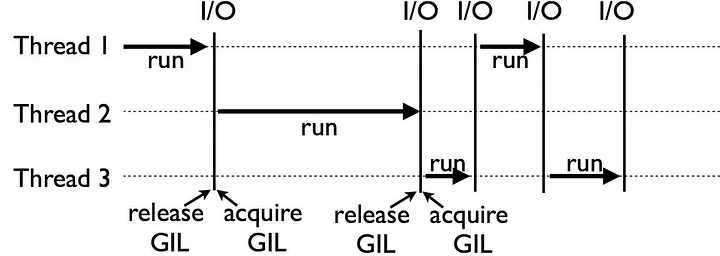
\includegraphics[width=\textwidth]{Chapitre4/figures/gil.png}
        \caption{Illustration of thread concurency in Python. The GIL prevents
            multiple threads from executing Python bytecodes in parallel.}
        \label{fig:gil}
    \end{figure}

    The GIL is not a problem for I/O bound applications. Threads can be used to handle I/O operations
    such as reading from a file, sending a request to a server, waiting for a response\dots
    The GIL is released when a thread is waiting for I/O. This allows other threads to execute Python
    bytecodes concurrently. Figure \ref{fig:gil} illustrates how the GIL affects thread concurrency in Python.


    The GIL, however, is a problem for CPU bound applications. Threads cannot be used to parallelize
    CPU bound tasks. The GIL prevents multiple threads from executing Python bytecodes at once.
    This means that a multi-threaded Python application will not be able to take advantage of multiple
    cores.\\

    A partial solution to the GIL problem is to use multiple processes instead of multiple threads.
    Each process will have its own Python interpreter and its own GIL. This allows multiple processes
    to run Python bytecodes in parallel. The multiprocessing module in Python provides a simple way
    to create multiple processes. However, the overhead of creating multiple processes can be significant.


    The benefit of using threads
    is that threads from the same process share the same memory space. This makes it easy to share objects
    between threads. Processes, on the other hand, do not share memory space. This complicates the sharing
    of data and introduces complex concepts in the code such as inter-process communication, shared memory\dots\\

    As our library is written internally in C++, we can benefit from the multi-threading capabilities
    of C++ from Python. Python code is not thread safe. However, out library's code is.
    Knowing this, we can make sure that when calling C++ code from Python, we release the GIL before
    invoking C++ code and acquire it back after the C++ code has finished executing. This way we can
    guarantee that Python bytecode is not executed in parallel while C++ code can run in parallel.\\

    As long as we do not alter Python objects in the C++ code, we can safely run C++ code in parallel
    from Python. This is a powerful feature that can be used to improve the performance of Python applications.

    This simple trick allowed us to run threaded code in Python in parallel working around the
    GIL limitations.

    \begin{figure}
        \centering
        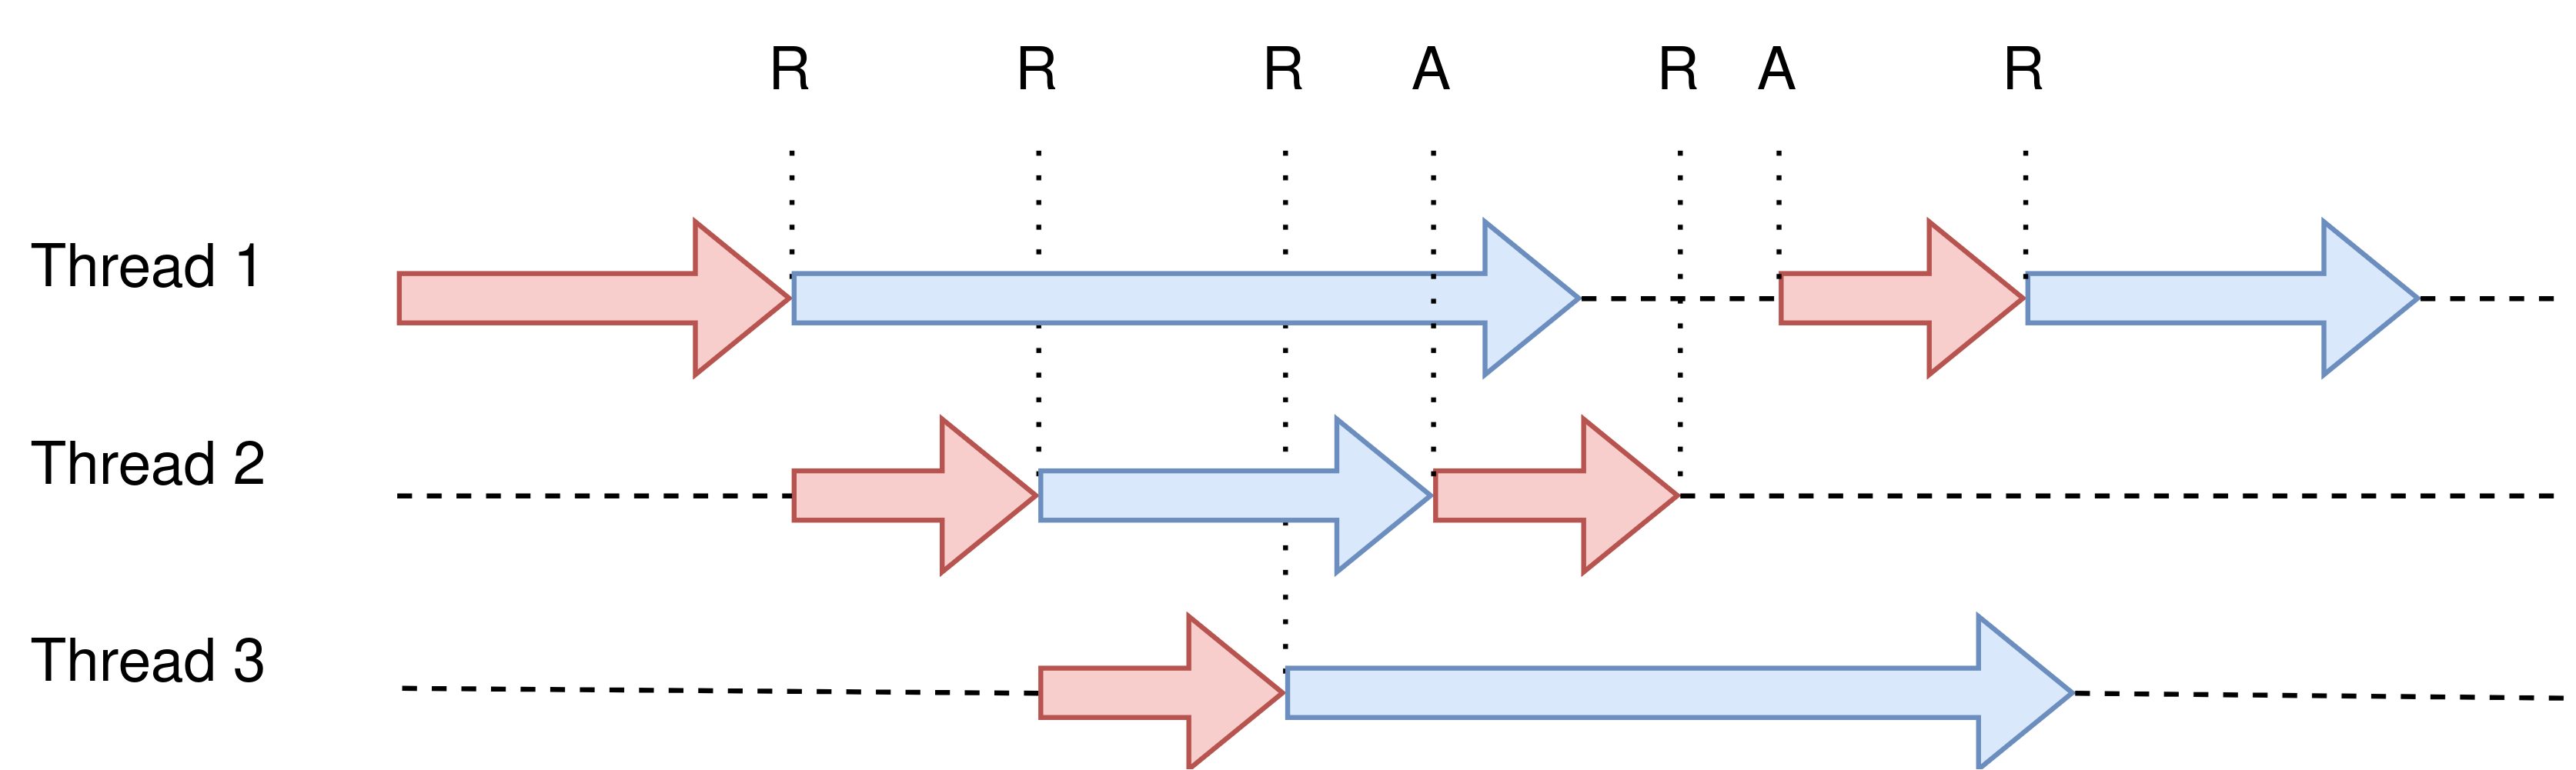
\includegraphics[width=\textwidth]{Chapitre4/figures/gil_c.png}
        \caption{Illustration of running multithreaded Python code with C++ bindings. Red arrows
            represent Python code, blue arrows represent C++ code. letter R represents releasing the GIL,
            letter A represents acquiring the GIL.}
        \label{fig:python_parallelization}
    \end{figure}

    Figure \ref{fig:python_parallelization} illustrates the execution of a multithreaded python code.
    As we can see from the figure, the GIL is released before invoking the C++ code and acquired back
    when running python code. Python code is not executed in parallel while C++ code can run in parallel.
    Effectively, we have bypassed the GIL limitations and achieved parallelization in multithreaded Python.

    \subsection{Performance Evaluation}
    In this subsection, the performance of different parallelization techniques will evaluated.
    As a benchmark, the common task of reading frames from a file, applying pedestal
    subtraction and finding clusters is used. This task contains I/O operations for reading frames from a file,
    and CPU bound operations for pedestal subtraction and cluster finding. We will evaluate the performance
    of the task using single threaded, multi-threaded and multi-process implementations.\\

    \subsubsection{Impact of the GIL}
    The python interface of the library uses C++ bindings to call the internal C++ code. As discussed in the previous section,
    the GIL prevents the parallelization of Python threads. Python threads run concurrently for IO bound tasks. However,
    for CPU bound tasks, the GIL prohibits the parallel execution of Python bytecodes.\\

    On the other hand, C++ code is thread safe and it is not affected by the GIL. For this reason, when calling C++ code
    from Python, we can release the GIL, run C++ code and acquire it back once the C++ code has finished executing. This way
    from Python's perspective the C++ code will treated the same as IO bound tasks and Python bytecodes will not be executed
    in parallel.\\

    To evaluate the impact of the GIL on our library we created two versions of the library. The first version releases the
    GIL before invoking the C++ code and the second one does not. We then ran the same task on both versions and compared the
    performance.\\

    \begin{table}
        \centering
        \begin{tabular}{|c|c|c|c|c|}
            \hline
            \multirow{2}{*}{\textbf{Thread Count}} & \multicolumn{2}{c|}{\textbf{GIL Acquired}} & \multicolumn{2}{c|}{\textbf{GIL Released}}                                          \\
                                                   & \textbf{Time (s)}                      & \textbf{CPU Usage}                        & \textbf{Time (s)} & \textbf{CPU Usage} \\
            \hline
            1                                      & 107                                    & 97\%                                      & 105               & 96\%               \\
            2                                      & 123                                    & 96\%                                      & 71                & 189\%              \\
            3                                      & 135                                    & 96\%                                      & 65                & 265\%              \\
            4                                      & 140                                    & 96\%                                      & 58                & 352\%              \\
            8                                      & 130                                    & 96\%                                      & 58                & 365\%              \\
            \hline
        \end{tabular}
        \caption{Impact of the GIL on the performance of the library. Comparing the time taken to run a task and the CPU usage
            on a 4-core machine.}
        \label{tab:gil_impact}
    \end{table}


    Table \ref{tab:gil_impact} shows the impact of the GIL on the performance of the library. The table compares the time
    taken to run a task and the CPU usage for different thread counts. The task was run on a 4-core machine. CPU usage is
    calculated as the sum of the CPU usage of all cores. As we can see from the table, the time taken to run the task is
    significantly higher when the GIL is present. The CPU usage is also lower with the GIL. This is because
    the GIL prevents the parallel execution of C++ code. As we use multiple threads we can see that the performance degrades
    as the number of threads increases. This is due to the cost of context switching between threads.\\

    In comparison when the GIL is not present, the time taken to run the task is significantly lower. CPU Usage quadrupled
    from 96\% to 365\%. The multiple threads are running in parallel and the performance improves as the number of threads
    increases. Figure \ref{fig:gil_impact} plots the table data. As we can see from the plot, the performance of the library
    is significantly improved when the GIL is released before calling C++ code.\\
    \begin{figure}
        \centering
        \subfloat[\centering Run Time]{{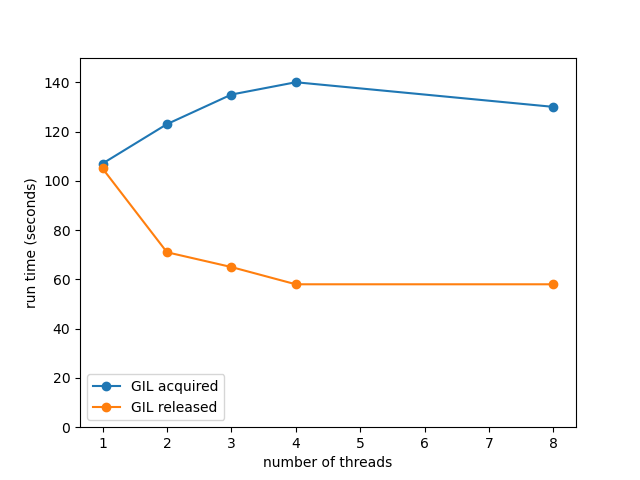
\includegraphics[width=0.8\textwidth]{Chapitre4/figures/gil1.png } }}%
        \qquad
        \subfloat[\centering CPU Usage]{{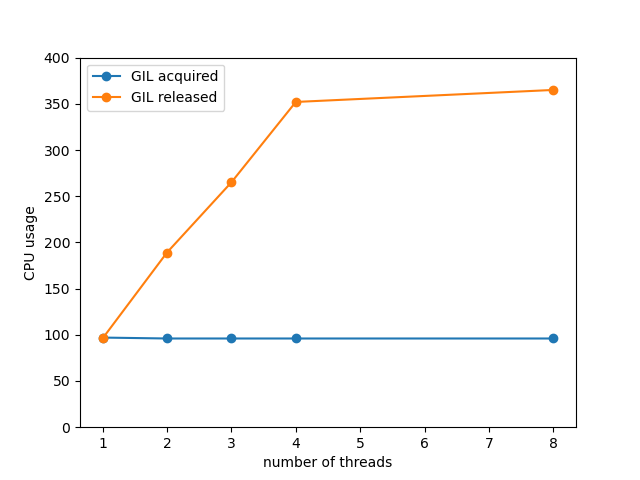
\includegraphics[width=0.8\textwidth]{Chapitre4/figures/gil2.png} }}%
        \caption{Plot showing the impact of releasing the GIL in the python bindings}%
        \label{fig:gil_impact}%


    \end{figure}

    Naturally, the performance of the C++ library is not affected by the GIL as it only impacts Python code.

    \subsubsection{Comparison of Different Parallelization Techniques}
    The next step is to compare the performance of different parallelization techniques. Four techniques are
    implemented: multi-threaded Python, multi-threaded C++, multi-process C++ with ZeroMQ, multi-threaded C++ with
    Producer and Consumer Queues.\\

    The experiments were done on a cloud virtual machine deployed on Azure Cloud. The machine used has  4 vCPUs and 16
    GB of RAM (D4s\_v3). The benchmark as previously defined is to read 8000 frames from a file, apply pedestal subtraction and
    find clusters.    \\

    Examples of the multi-threaded C++ and Python implementations are shown in listings \ref{lst:multi_threaded_cpp} and
    \ref{lst:multi_threaded_python}. The same idea is implemented exactly in python and in C++. In these examples
    a list of functions is created. Each function reads a different set of frames from the file independently from
    the others. These functions will then be run in threads in parallel.\\

    The multi-threaded C++ with Producer and Consumer Queues implementation is similar to the multi-threaded C++ implementation.
    The difference is that instead of running the functions in threads directly, a thread will push frames to a queue and
    other threads will pop frames from the queue and process them. This is a common pattern used in multi-threaded applications.
    In our comparison it serves as a reference point to compare the performance of the other implementations.\\

    The multi-process C++ with ZeroMQ implementation is based on the task distribution model implemented in the library.
    The ventilator, worker, sink model is designed to work over the network but it can also be used to distribute tasks
    to multiple processes on the same machine. The ventilator will read frames from the file and send them to the workers
    over ZeroMQ. All communications will be local to the host machine and will not go over the network.\\


    \begin{lstlisting}[language=C++, caption=Multi-threaded C++ example, label=lst:multi_threaded_cpp]
const int N_FRAMES = 8000;
std::filesystem::path fname;

std::function<void()> thread_function_factory(int offset, int step) {
    // return a function that will be run in parallel
    // the function has a closure over the offset and step
    // in case of 4 threads, step will be equal to 4 and offset will be 0,1,2,3
    // the function reads frames from the file starting from the offset and reads every step-th frame
    // one function will read frames 0,4,8,12... another will read frames 1,5,9,13...
    return [offset, step]() {
        Pedestal<double> pedestal(400, 400, 1000); // create pedestal object
        File file(fname, "r"); // open file
        ClusterFinder cf(3, 3, 5, 0); // inialize cluster finder
        for (int i = offset; i < N_FRAMES; i += step) {
            // read frame and run cluster finder algorithm
            auto frame = file.iread(i); 
            auto clusters = cf.find_clusters_without_threshold(frame.view<uint16_t>(), ped, false);
        }
    };
}
    \end{lstlisting}

    \begin{lstlisting}[language=Python, caption=Multi-threaded Python example, label=lst:multi_threaded_python]
# function that will be run in parallel
def executor(offset,n_threads):
    file = File(file_path)
    pedestal = Pedestal(400,400,1000)
    cf = ClusterFinder(3,3,5.0,0)
    for i in range(offset,N_FRAMES,n_threads):
        frame = file.iread(i)
        clusters=cf.find_clusters_without_threshold(frame,pedestal,False)

    

thread_arr = []
for i in range(N_THREADS):
    # create and run threads
    thread_arr.append(Thread(target=executor,args=(i,N_THREADS)))
    thread_arr[i].start()
    \end{lstlisting}



    \begin{table}
        \centering
        \begin{tabular}{|c|c|c|c|c|}
            \hline
            \textbf{Thread/Process Count} & \textbf{MT C++} & \textbf{MT Python} & \textbf{MT C++ PCQ} & \textbf{MP C++ ZMQ} \\
            \hline
            1                     & 74              & 98                 & 90                  & 143                 \\
            2                     & 37              & 51                 & 46                  & 72                  \\
            3                     & 37              & 49                 & 46                  & 70                  \\
            4                     & 35              & 50                 & 47                  & 67                  \\
            8                     & 36              & 47                 & 43                  & 68                  \\
            \hline
        \end{tabular}
        \caption{Comparison of different parallelization techniques. Time taken to run the benchmark in seconds.
            MT C++: Multi-threaded C++, MT Python: Multi-threaded Python, MT C++ PCQ: Multi-threaded C++ with Producer and
            Consumer Queues, MP C++ ZMQ: Multi-process C++ with ZeroMQ.}
        \label{tab:parallelization_comparison}
    \end{table}
    \begin{figure}
        \centering
        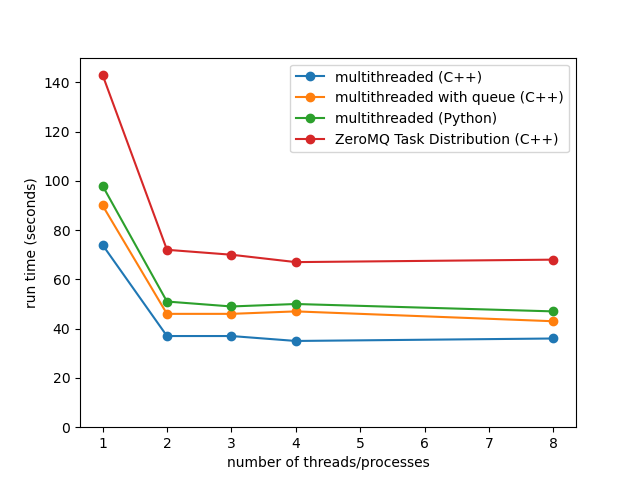
\includegraphics[width=\textwidth]{Chapitre4/figures/comp.png}
        \caption{Comparison of different parallelization techniques. Time taken to run the benchmark in seconds.}
        \label{fig:parallelization_comparison}
    \end{figure}

    Table \ref{tab:parallelization_comparison} and figure \ref{fig:parallelization_comparison} show the time taken to run the
    benchmark for different parallelization techniques. The multithreaded C++ example is the fastest. It took 35 seconds to run 
    the test on 4 threads. Naturally, the multi-process ZeroMQ example is the slowest. It is always twice slower than the
    multi-threaded C++ example.\\

    Surprisingly, python performed close results to C++. The multi-threaded Python example took 47 seconds to run on 8 threads.
    While the producer consumer C++ example took 43 seconds. Compared to the multithreaded C++ example, it is in general 35\% 
    slower. This is a good result for Python! This is orders of magnitude faster than code written in pure Python.\\ 

    When designing the library, it was first thought that the same task distribution model could be used as a parallelization
    framework locally. The results of this evaluation show that the model is not as efficient as a multi-threaded implementation
    in C++. As much as it is convenient if we could reuse the same code to scale it horizontally and vertically it is not
    practical. On the other hand multi-threaded code proved itself as the most efficient way to parallelize and it comes 
    with the least overhead.\\
    \section*{Conclusion}
    In this chapter we explored different use cases of the library. We demonstrated the flexibility and power of the library
    by combining its components to realize different applications. We also discussed the parallelization features 
    and benchmarked its performance with various parallelization techniques. The results show that the library is
    efficient and can be used to handle complex tasks in simple ways and with high performance.\\

    %==============================================================================
\end{spacing}
